\documentclass[11pt]{article}
\usepackage[margin=2.2cm]{geometry}
\usepackage{amsmath,amssymb,booktabs,array}
\usepackage[T1]{fontenc}
\usepackage{lmodern}
\usepackage{tikz}
\usetikzlibrary{arrows.meta,decorations.pathreplacing,calc}
\setlength{\parskip}{0.5em}\setlength{\parindent}{0pt}
\title{Out-of-fold predictions and calibration\\of the discrete-time hazard model}
\author{MASTU\_hazard notes}
\date{}
\begin{document}
\maketitle

This note explains what \texttt{hazard\_predict.py --pooled} checks and why the
checks are valid. It covers what a prediction means
(\S\ref{sec:row}), where the predictions come from (\S\ref{sec:oof}), and the
calibration check step by step (\S\ref{sec:cal}--\ref{sec:read}). The other two
plots, the aligned hazard and the shot separation, are in \S\ref{sec:other}.

%-----------------------------------------------------------------------------
\section{What one prediction means}\label{sec:row}

The survival table has one row per equilibrium slice. Row $i$ belongs to shot
$s_i$ at time $t_i$ and carries features $x_i$. Its label is $y_i=1$ only on
the last slice before onset; every other row has $y_i=0$. A shot's rows stop at
onset, so each shot has at most one $y=1$. Shots with no onset are
\emph{censored}: all of their rows have $y=0$.

The model returns, for each row, a number $p_i\in(0,1)$:
\[
p_i \;=\; \Pr\bigl(\text{onset in } (t_i,\,t_i+\Delta t] \;\big|\; \text{no onset by } t_i,\; x_i\bigr),
\qquad
h_i = p_i/\Delta t \;\;[\mathrm{s}^{-1}] .
\]
Here $\Delta t$ is the slice cadence (the \texttt{dt} that \texttt{merge\_pair}
measures, about 5\,ms on EPM). $h$ is the hazard rate. The probability that a
shot survives to time $t$ is
\[
S(t)=\prod_{t_i\le t}(1-p_i).
\]

\paragraph{Why each row can be treated as a coin flip.}
The likelihood of one shot is ``survive each slice, then (maybe) have onset in
the last one'':
\[
L_{\text{shot}}=\prod_{i\in\text{shot}} p_i^{\,y_i}(1-p_i)^{1-y_i}.
\]
This is exactly the likelihood of independent Bernoulli trials, one per row.
That is why the per-row logistic loss \emph{is} the survival likelihood (the
\texttt{hazard\_model} docstring), and it is also why every row-level check
below is legitimate.

Rows of one shot are strongly correlated in their \emph{features}. But if the
model is right, each $y_i$ is a coin flip with probability $p_i$, given
everything before it. So a sum $\sum y_i$ over any set of rows has mean
$\sum p_i$ and variance $\sum p_i(1-p_i)$, whichever shots the rows come
from.\footnote{Strictly: $\sum (y_i-p_i)$ is a martingale sum, so its
variance is the sum of the conditional variances. Correlations between
features do not enter.}

%-----------------------------------------------------------------------------
\section{\texttt{oof}: out-of-fold, not out-of-distribution}\label{sec:oof}

\textbf{oof} stands for \emph{out-of-fold}. It has nothing to do with OOD
(out-of-distribution).

\texttt{hazard\_model.py} splits the \emph{shots} into $K=8$ groups. For each
group $k$ it trains a model on the other seven groups and predicts the rows of
group $k$. After eight fits every row has exactly one prediction, made by a
model that never saw any slice of that shot. The column of these predictions is
\texttt{oof}.

\begin{center}
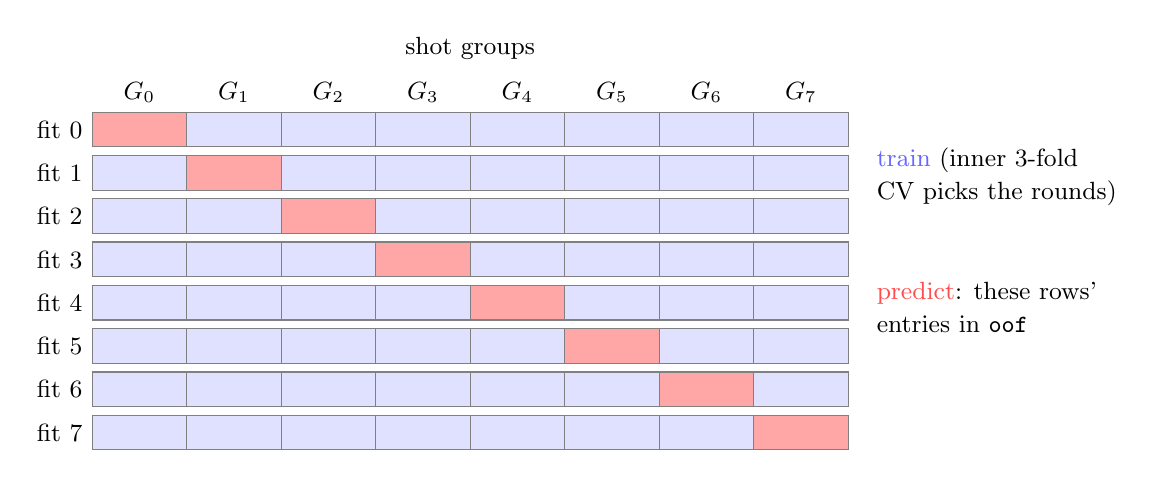
\begin{tikzpicture}[x=1.2cm,y=0.55cm]
  \node[above] at (4,1.0) {\small shot groups};
  \foreach \k in {0,...,7} {
    \foreach \j in {0,...,7} {
      \ifnum\j=\k
        \fill[red!35] (\j,-\k) rectangle ++(1,-0.8);
      \else
        \fill[blue!12] (\j,-\k) rectangle ++(1,-0.8);
      \fi
      \draw[gray] (\j,-\k) rectangle ++(1,-0.8);
    }
    \node[left] at (0,-\k-0.4) {\small fit $\k$};
  }
  \foreach \j in {0,...,7} \node[above] at (\j+0.5,0) {\small $G_\j$};
  \node[right,align=left] at (8.2,-1.5) {\small\textcolor{blue!60}{train} (inner 3-fold\\ \small CV picks the rounds)};
  \node[right,align=left] at (8.2,-4.5) {\small\textcolor{red!70}{predict}: these rows'\\ \small entries in \texttt{oof}};
\end{tikzpicture}
\end{center}

\paragraph{Why oof predictions are needed.}
A boosted tree scored on its own training rows looks better than it is, because
it has partly memorised them. In particular, its predictions there are too
extreme: too high on event rows, too low elsewhere. Calibration measured on
training rows would therefore be meaningless. On oof rows every prediction is
an honest test.

\paragraph{Three things to keep in mind.}
\begin{enumerate}
\item \texttt{oof} is stitched together from eight \emph{different} models.
  Calibration on \texttt{oof} grades the fitting procedure, i.e.\ what a model
  trained this way does on unseen shots. It does not grade one particular
  model.
\item With \texttt{--repeats} $B>1$ the whole 8-fold split is redone with fresh
  shot groupings, and \texttt{oof} has $B$ columns. \texttt{hazard\_predict}
  averages them; their spread is the band in the per-shot traces.
\item oof shots come from the \emph{same} campaign and the same annotation as
  the training shots. This is not a distribution-shift test. Running the
  stored fold models on another campaign would be (the per-shot mode, not yet
  written).
\end{enumerate}

%-----------------------------------------------------------------------------
\section{Calibration, step by step}\label{sec:cal}

\paragraph{The definition.}
The model is \emph{calibrated} if, among all rows where it says $p$, a fraction
$p$ actually have onset:
\[
\Pr(y=1 \mid \hat p = q) = q \quad\text{for every } q .
\]
This is what entitles us to read $p/\Delta t$ as a rate in s$^{-1}$, and $S(t)$
as a probability.

\paragraph{Why binning is needed.}
The definition cannot be checked one value of $q$ at a time. $p$ is continuous,
so no two rows share exactly the same $p$, and each row's outcome is just 0 or
1. A single row with $p=0.03$ and $y=0$ tells us almost nothing. So rows with
\emph{similar} $p$ are pooled, and their average prediction is compared with
the fraction that had onset. That pooling is all the ``binning'' is.

\paragraph{The recipe} (\texttt{hazard\_predict.calibration}):
\begin{enumerate}
\item Sort all $N$ rows by predicted $p$.
\item Cut the sorted list into $G$ consecutive groups of equal size, $N/G$ rows
  each (default $G=10$).
\item For each group $g$, compute:
  \[
  n_g=\#\text{rows},\qquad
  \bar p_g = \frac{1}{n_g}\sum_{i\in g}p_i ,\qquad
  \hat E_g=\sum_{i\in g}p_i = n_g\bar p_g,\qquad
  E_g = \sum_{i\in g}y_i,\qquad
  r_g = E_g/n_g .
  \]
  $\hat E_g$ is the number of onsets the model \emph{expects} in the group; $E_g$
  is the number \emph{observed}.
\item Plot one point per group at $(\bar p_g,\; r_g)$, with an error bar on
  $r_g$. A calibrated model puts the points on the diagonal $r=\bar p$, within
  the error bars. Equivalently, $E_g\approx\hat E_g$.
\end{enumerate}

\begin{center}
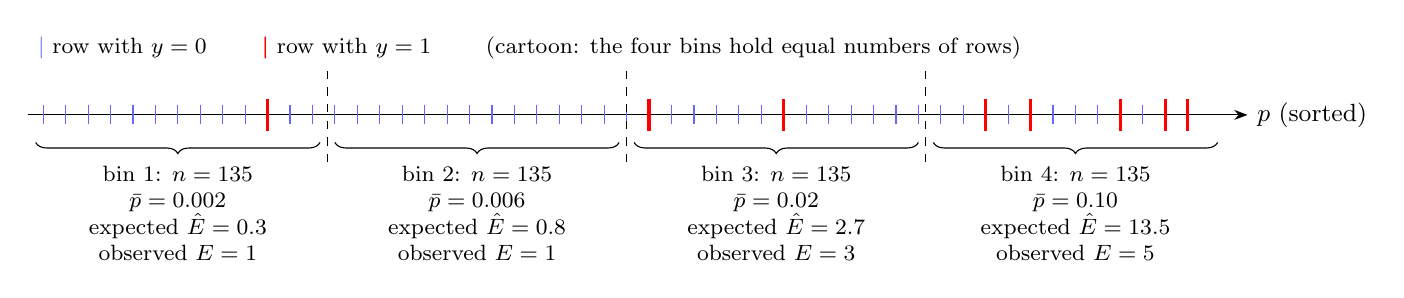
\begin{tikzpicture}[x=0.95cm,y=1cm]
  % sorted rows
  \draw[-{Stealth}] (0,0) -- (16.3,0) node[right] {\small $p$ (sorted)};
  \foreach \x in {0.2,0.5,...,15.8} \draw[blue!60] (\x,-0.12) -- (\x,0.12);
  \foreach \x in {3.2,8.3,10.1,12.8,13.4,14.6,15.2,15.5}
     \draw[red,very thick] (\x,-0.2) -- (\x,0.2);
  \foreach \b in {4,8,12} \draw[dashed] (\b,-0.6) -- (\b,0.6);
  \foreach \b/\lab/\pb/\Eh/\E in {0/1/0.002/0.3/1,4/2/0.006/0.8/1,8/3/0.02/2.7/3,12/4/0.10/13.5/5}{
     \draw[decorate,decoration={brace,mirror,amplitude=4pt}] (\b+0.1,-0.35) -- (\b+3.9,-0.35);
     \node[align=center,font=\footnotesize] at (\b+2,-1.25)
       {bin \lab: $n=135$\\ $\bar p=\pb$\\ expected $\hat E=\Eh$\\ observed $E=\E$};
  }
  \node[font=\footnotesize,anchor=west] at (0,0.85)
    {\textcolor{blue!60}{$|$} row with $y=0$ \qquad \textcolor{red}{$\boldsymbol|$} row with $y=1$
     \qquad (cartoon: the four bins hold equal numbers of rows)};
\end{tikzpicture}
\end{center}

In the cartoon, bin 4 expects 13.5 onsets and sees 5. The model is too high
there. Bins 1--3 agree within counting noise.

\paragraph{Why equal-count bins, and why log axes.}
Onset is rare: the base rate per 5\,ms slice is of order $10^{-2}$. Most rows
have $p\sim10^{-3}$, and a few have $p\sim10^{-1}$. Equal-\emph{width} bins on
$[0,\max p]$ would put almost every row into the first bin and leave the rest
nearly empty. Equal-\emph{count} bins follow the rows, so every point has the
same number of rows behind it. Because $p$ spans two to three decades, both
axes are logarithmic. The histogram under the calibration plot shows where the
rows actually are, with the bin edges marked.

\paragraph{Error bars.}
Given the model, $E_g$ is a sum of independent coin flips
(\S\ref{sec:row}). It has
\[
\mathbb E[E_g]=\hat E_g, \qquad \operatorname{Var}E_g=\sum_{i\in g}p_i(1-p_i)\;\le\;n_g\bar p_g(1-\bar p_g) .
\]
So the binomial distribution with parameters $(n_g,\bar p_g)$ is a slightly
conservative yardstick. The plot shows the 68\% Wilson interval for $r_g$:
\[
\frac{\hat r+\frac{z^2}{2n}\;\pm\; z\sqrt{\frac{\hat r(1-\hat r)}{n}+\frac{z^2}{4n^2}}}{1+\frac{z^2}{n}},
\qquad \hat r = E_g/n_g,\; z=1 .
\]
The Wilson form is used because the simple $\hat r\pm\sqrt{\hat r(1-\hat r)/n}$
collapses to zero width when $E_g=0$, which is common in the low-$p$ bins. A
bin with no onsets is drawn as a red triangle at the bottom of the plot; its
interval still has a positive upper end. The \emph{relative} error is roughly
$1/\sqrt{E_g}$. With a few hundred events spread over ten bins, the low bins
hold only a handful each, so expect visible scatter there. That scatter is
counting noise, not miscalibration.

\paragraph{The two summary numbers.}
\begin{itemize}
\item \emph{Calibration in the large:} total observed events $\sum_g E_g$
  against total expected $\sum_i p_i$. A mismatch means the overall level is
  off, e.g.\ the base rate differs between the training folds and the test
  folds.
\item \emph{Hosmer--Lemeshow:}
  \[
  \mathrm{HL}=\sum_{g=1}^{G}\frac{(E_g-\hat E_g)^2}{\hat E_g\,(1-\bar p_g)} .
  \]
  This is a $\chi^2$-type sum of squared standardised misses. For a calibrated
  model it is roughly $\chi^2$ with $G-2$ degrees of freedom: mean $G-2$,
  standard deviation $\sqrt{2(G-2)}$, i.e.\ $8\pm4$ for ten bins. Treat it as a
  flag, not a p-value. The $\chi^2$ approximation is poor when $\hat E_g<5$,
  which happens in the low bins, and HL changes with $G$.
\end{itemize}

%-----------------------------------------------------------------------------
\section{Reading the calibration plot}\label{sec:read}

\begin{center}
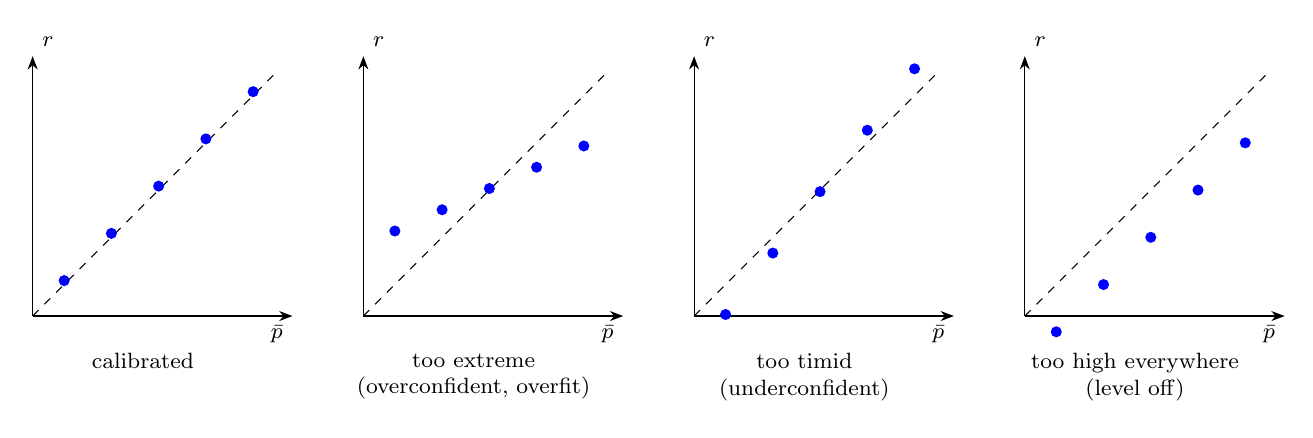
\begin{tikzpicture}[x=1cm,y=1cm,font=\footnotesize]
  \def\panel#1#2#3{%
    \begin{scope}[shift={(#1,0)}]
      \draw[-{Stealth}] (0,0) -- (3.3,0) node[below left] {$\bar p$};
      \draw[-{Stealth}] (0,0) -- (0,3.3) node[above right] {$r$};
      \draw[dashed] (0,0) -- (3.1,3.1);
      #2
      \node[align=center,anchor=north] at (1.4,-0.35) {#3};
    \end{scope}}
  \panel{0}{\foreach \x in {0.4,1.0,1.6,2.2,2.8} \fill[blue] (\x,\x+0.05) circle (2pt);}{calibrated}
  \panel{4.2}{\foreach \x in {0.4,1.0,1.6,2.2,2.8} \fill[blue] (\x,{0.9+0.45*\x}) circle (2pt);}{too extreme\\(overconfident, overfit)}
  \panel{8.4}{\foreach \x in {0.4,1.0,1.6,2.2,2.8} \fill[blue] (\x,{-0.5+1.3*\x}) circle (2pt);}{too timid\\(underconfident)}
  \panel{12.6}{\foreach \x in {0.4,1.0,1.6,2.2,2.8} \fill[blue] (\x,{\x-0.6}) circle (2pt);}{too high everywhere\\(level off)}
\end{tikzpicture}
\end{center}

\begin{itemize}
\item \textbf{Points below the diagonal:} the model predicts more onsets than
  occur. \textbf{Above:} fewer.
\item \textbf{Flatter than the diagonal} (below it at high $p$, above it at low
  $p$): the predictions are too extreme. This is the usual signature of
  overfitting. More regularisation (larger \texttt{min\_child\_weight}, smaller
  \texttt{max\_depth}) or fewer rounds pulls the points onto the diagonal.
\item \textbf{Steeper than the diagonal:} the predictions are too timid. The
  model is under-using what it has learned.
\item \textbf{Parallel offset:} the overall level is wrong. Calibration in the
  large shows the same thing.
\end{itemize}

\paragraph{Calibration is not the same as being useful.}
The shuffled-target control, or a model that always returns the base rate $p_0$,
is \emph{perfectly calibrated}: all its rows fall in one cloud at $(p_0,p_0)$,
on the diagonal. It is also useless, because it cannot tell one slice from
another. The spread of the points \emph{along} the diagonal is what shows
discrimination. A good model is calibrated \emph{and} spreads the rows over
decades in $p$. The test log-likelihood gain that \texttt{hazard\_model} prints
rewards both at once. The plots in \S\ref{sec:other} show discrimination
directly.

\paragraph{A worked example (synthetic).}
This example comes from the offline test generator, not MAST-U data:
$600$ shots, 24\,016 rows, 320 onsets, $\Delta t=5$\,ms, 8 folds $\times$ 2
repeats. \texttt{hazard\_predict} printed:
\begin{center}\footnotesize
\begin{tabular}{rrrrrr}
\toprule
bin & rows & $\bar p$ & expected $\hat E$ & observed $E$ & $r=E/n$ \\
\midrule
0 & 2402 & $1.22\times10^{-3}$ & 2.94 & 2 & $8.3\times10^{-4}$\\
2 & 2402 & $1.92\times10^{-3}$ & 4.62 & 1 & $4.2\times10^{-4}$\\
5 & 2402 & $3.66\times10^{-3}$ & 8.80 & 11 & $4.6\times10^{-3}$\\
7 & 2401 & $8.66\times10^{-3}$ & 20.79 & 16 & $6.7\times10^{-3}$\\
8 & 2401 & $2.11\times10^{-2}$ & 50.57 & 58 & $2.4\times10^{-2}$\\
9 & 2401 & $8.74\times10^{-2}$ & 209.73 & 214 & $8.9\times10^{-2}$\\
\bottomrule
\end{tabular}
\end{center}
(six of the ten bins shown). In total, 320 onsets were observed against 325.6
expected, and HL $=11.0$ against $8\pm4$: calibrated. Bin 2 sees 1 onset where
4.6 are expected, which looks bad as a ratio. But with Poisson noise
$\sqrt{4.6}\approx2.1$ it is only 1.7$\sigma$ low. The top bin holds two
thirds of all onsets, and its $\bar p$ is 70 times that of bin 0. That spread is
the discrimination.

%-----------------------------------------------------------------------------
\section{The other two pooled plots}\label{sec:other}

\paragraph{Aligned hazard.}
For each event shot, every row is given its time before onset,
$\tau=t_{\text{onset row}}-t_i$. For each censored shot, every row is given its
time before the shot's last row. Rows are then binned in $\tau$ (default
$2\Delta t$), and the median and interquartile range of $h$ are drawn against
$\tau$ for each class. If the model has learned precursors, the event curve
rises above the censored curve as $\tau\to0$. The $\tau$ at which the two
curves separate is the model's typical warning time. The censored reference
point is simply the end of the analysis window, not a physical event.

\paragraph{Shot separation.}
For each shot this plot takes the peak $h$ over its rows, then compares the
event-shot and censored-shot histograms. The AUC is the probability that a
randomly chosen event shot peaks higher than a randomly chosen censored one
(0.5 means no separation, 1 means perfect). It is computed by ranks
(Mann--Whitney), with ties counted half. One caveat: event shots stop at
onset, while censored shots run to the end of the window and so have more rows
over which to reach a high peak. This biases the AUC \emph{down}, which makes
it a conservative number.

\end{document}
